\documentclass[10pt]{article}
\usepackage[utf8]{inputenc}
\usepackage[activeacute,spanish,es-nodecimaldot]{babel}
\usepackage[left=1.5cm,top=1.5cm,right=1.5cm, bottom=1.5cm,letterpaper, includeheadfoot]{geometry}
\usepackage[parfill]{parskip}

\usepackage{amssymb, amsmath, amsthm}
\usepackage{graphicx}
\usepackage{lmodern,url}
\usepackage{paralist} %util para listas compactas

\usepackage{fancyhdr}
\pagestyle{fancy}
\fancypagestyle{plain}{%
\fancyhf{}
\lhead{\footnotesize\itshape\bfseries\rightmark}
\rhead{\footnotesize\itshape\bfseries\leftmark}
}


% macros
\newcommand{\Q}{\mathbb Q}
\newcommand{\R}{\mathbb R}
\newcommand{\N}{\mathbb N}
\newcommand{\Z}{\mathbb Z}
\newcommand{\C}{\mathbb C}

%Teoremas, Lemas, etc.
\theoremstyle{plain}
\newtheorem{teo}{Teorema}
\newtheorem{lem}{Lema}
\newtheorem{prop}{Proposición}
\newtheorem{cor}{Corolario}

\theoremstyle{definition}
\newtheorem{defi}{Definición}

%implica y equivale
\newcommand{\ssi}{\Longleftrightarrow}
\newcommand{\imp}{\implies}
% fin macros

%%%%% NOMBRE ESCRIBAS Y FECHA
\newcommand{\sca}{Juan Pablo Donoso Merlet}
\newcommand{\scb}{Escriba Dos}
\newcommand{\scc}{Escriba Tres}
\newcommand{\catnum}{0} %numero de catedra
\newcommand{\fecha}{12 de marzo 2018 }

%%%%%%%%%%%%%%%%%%

%Macros para este documento
\newcommand{\cin}{\operatorname{cint}}


\begin{document}
%Encabezado
\fancyhead[L]{Facultad de Ciencias Físicas y Matemáticas}
\fancyhead[R]{Universidad de Chile}
\vspace*{-1.2 cm}
\begin{minipage}{0.6\textwidth}
\begin{flushleft}
\hspace*{-0.5cm}\textbf{MA4702. Programación Lineal Mixta. 2018.}\\
\hspace*{-0.5cm}\textbf{Profesor:} José Soto\\
\hspace*{-0.5cm}\textbf{Escriba(s):} \sca\\
\hspace*{-0.5cm}\textbf{Fecha:} \fecha.
\end{flushleft}
\end{minipage}
\begin{minipage}{0.36\textwidth}
\begin{flushright}

\includegraphics[scale=0.15]{fcfm}
\end{flushright}
\end{minipage}
\bigskip
%Fin encabezado

\begin{center}
\LARGE\textbf{Cátedra \catnum}
\end{center}

%\section{Escribiendo apuntes con \LaTeX}
%
%En la red hay bastante material para aprender a usar esta herramienta. Como ejemplo, les recomiendo visitar
%\url{http://latex-project.org/guides/} y \url{http://texblog.net/}.
%
%Además, es bueno empezar a seguir buenas prácticas, dejando de lado un montón de comandos que están obsoletos (en particular, reemplazar \verb+\eqnarray+ y \verb+$$ ... $$+ por los más modernos \verb+\align+ y \verb+\[ ... \]+).
%
%\subsection{Recomendaciones para escribir un apunte}
%Es bueno comenzar cada clase con una frase introductoria, explicando lo que se va a ver. No llegue y copie textualmente lo que se ve en la pizarra sin incorporar comentarios que aclaren (en clases, suelo decir mucho más de lo que escribo).
%
%Recuerde que las ecuaciones también son parte del texto, y luego deben cumplir las reglas de puntuación (por ejemplo, usar comas y puntos
%finales).
%
%\subsection{Algunos ejemplos}
%
%\subsubsection*{Uso simple de macros:}
%\begin{defi}[Cintura de un grafo]
% La \emph{cintura} de un grafo es el largo del ciclo más corto. Si el grafo es acíclico, se define como $+\infty$.
%Denotaremos la cintura de $G$ por $\cin(G)\in \Z$. 
%\end{defi}
%Observar (en la fuente) la definici\'on de las macros \verb+\Z+ y \verb+\cin+.
%
%\begin{lem}
% Si $G$ es un grafo bipartito entonces $\cin(G)\ge 3$.
%\end{lem}
%
%M\'as ejemplos: Escriba $\min(X)$ (\begin{verb}$\min(X)$\end{verb}) en vez de $min(X)$ (el \'ultimo parece producto de $m$, $i$ y $n$). 
%Por lo mismo, escriba tambi\'en $X_{\text{opt}}$ (\begin{verb}$X_{\text{opt}}$\end{verb}) en vez de $X_{opt}$.
%
%
%\subsubsection*{Ecuaciones alineadas.}
%
%No es difícil escribir ecuaciones que tengan una sola alineación como
%\begin{align}
%\psi(n)
%&= \frac{(2n)!}{n! 2^n} = \frac{(2n)(2n-1) \dotsm (n+1)}{2^n} \notag \\
%&\geq \left( \frac{n}{2} \right)^n. \label{eqn:interesante}
%\end{align}
%
%Sin embargo, escribir un PL en \LaTeX{} puede ser complicado. Un formato tipo para escribir simultáneamente un primal y un dual es el siguiente:
%
%\begin{alignat*}{5}
%&\max\        & \sum_{ij \in E} x_{ij}w_{ij} &		 &                      &\qquad\qquad \min\        &\sum_{i \in V}y_i&\\
%&\text{s.a. } & \sum_{j\colon j\neq i} x_{ij}&\leq 1 &\quad\forall i \in V  &\qquad\qquad \text{s.a. } &y_i+y_j &\geq w_{ij} &\quad\forall ij \in E\\
%&	          & x_{ij}                       &\geq 0 &\quad\forall ij \in E &\qquad\quad               &y_i &\geq 0      &\quad\forall i \in V.
%\end{alignat*}
%
%\medskip
%Este es solo un documento de ejemplo. Entre otras cosas \LaTeX{} permite escribir fácilmente
%\begin{itemize}
%  \item Matrices.
%  \item Integrales.
%  \item Tablas.
%  \item Listas.
%  \item etc.
%\end{itemize}
\section{PLM: Modelos y formulaciones.}
\subsection*{Modelos}
Partamos con definiciones elementales:\\
\begin{defi}[Problema de optimización e instancias]
Un \textit{problema de optimización} $(P)$ consiste en un conjunto de \textit{instancias}, siendo una \textit{instancia} definida por tres aspectos:
\begin{itemize}
\item Un conjunto factible $S$.
\item Una función a optimizar $f: S \to \R$.
\item Un objetivo, minimizar o maximizar la función $f$ en dicho conjunto $S$.
\end{itemize}
\end{defi}
~\\
Por ejemplo, para  el problema de optimización de MST, una instancia estaría conformada por un grafo $G = (V,E)$ con pesos en las aristas, junto con un conjunto factible  $S$ de los árboles generadores de dicho grafo $G$.\\

\underline{\textbf{observación}}: Diremos que \textit{resolvemos} una instancia siempre y cuando seamos capaces de realizar alguna de las dos siguientes opciones:\\

\begin{enumerate}
\item Encontrar $\text{OPT} \in S$ tal que $f(OPT) = \max_{x \in S} f(x)$

\item Mostrar que no hay un elemento $OPT \in S$ que cumpla lo anterior, donde en general hay tres casos:
\begin{itemize}
\item Por infactibilida ($S  = \emptyset$).
\item El problema es no acotado (máximo es $+ \infty$).
\item No alcanzable, i.e. el máximo no se alcanza pero si supremo.
\end{itemize}
\end{enumerate}
~\\
Por último, recordemos lo que es un \textit{algoritmo}.\\
\begin{defi}[Algoritmo]
Una secuencia de instrucciones que resuelve \textit{instancias} de un problema de optimización $(P)$.
\end{defi}

Así, los problemas que nos interesarán en este curso son aquellos que se puedan \textit{modelar} como un PLM.\\

\begin{defi}[PLM]
Un Programa Lineal Mixto consiste es un problema de optimización tal que el conjunto factible $S$ es un \textit{conjunto lineal mixto}, es decir:
$$
S := \{x \in \Z^E \times \R^C: Ax \leq b \} \subseteq \R^n
$$
con $n, m \in \N$, $E$,$C \subseteq [n]$ tales que $E \cup C = [n]$, $A \in \mathcal{M}_{m \times n}(\R)$ y $b \in \R^m$.\\
\end{defi}

\textbf{Ejemplo:}(Knapsack)\\ 

Consideremos el siguiente problema. Tenemos $n \in \N$ objetos, cada uno con un valor $v_i \geq 0$ y tamaño $s_i \geq 0$ asociados, y una mochila de capacidad $B \geq 0$. La  idea es seleccionar los objetos a poner en la mochila de modo tal de maximizar el valor total, i.e.:
\begin{alignat*}{5}
&\max\        & \sum_{i \in [n]} v_i x_i \\
&\text{s.a. } & \sum_{i \in [n]} s_i x_i&\leq B &  \\
&                  & x_i                       &\in \{0,1\} &\quad\forall i \in [n] 
\end{alignat*}

Notar que el vector $x \in \{0,1\}^n$ es tal que:
$$
x_i =1 \ssi \text{el objeto $i$ se agrega a la mochila.}
$$\\

\underline{\textbf{observación}}: La palabra \textit{modelo} se usa muy coloquialmente como algo intercambiable con \textit{formulación}. En rigor:

\begin{center}
\textit{Un PLM es un modelo de una instancia si podemos extraer una solución de dicha instancia resolviendo el PLM}
\end{center}

Así, lo mínimo que se pedirá a un PLM en la modelación de un problema es:
\begin{itemize}
\item Óptimos del PLM se asocian a optimos del problema.
\item Algún óptimo del problema se refleje como objeto factible del PLM.
\end{itemize}
Por último, si pidiesemos que el conjunto factible del PLM fuese \textbf{igual} al conjunto de soluciones factibles del problema, hablamos de un problema exacto.\\

\textbf{Ejemplo:} El modelo de knapsack es exacto.\\

\textbf{Ejemplo (de problema no exacto):} Caminos de largo mínimo en un grafo dirigido. Sea $G = (V, \vec{E})$ un digrafo, con un nodo origen $s \in V$ y un nodo destino $t \in V$. Consideremos además una función de largos no negativos $\ell: \vec{E} \to \R_+$.  Veamos este problema de dos maneras:
\begin{enumerate}
\item \textbf{Como flujo:} El problema de optimización a resolver es:
\begin{alignat*}{5}
&\min\        & \sum_{\vec{e} \in \vec{E}} \ell_{\vec{e}} x_{\vec{e}} \\
&\text{s.a. } & x(\delta^-(v))-x(\delta^+(v))&= \begin{cases}0 & v \not \in  \{s,t\}\\ -1 & \mbox{si } v=s\\1 & \mbox{si } v=t \end{cases}, &  \quad\forall v \in V\\
&                  & x_{\vec{e}}                      &\in \{0,1\} &\quad\forall \vec{e} \in \vec{E} 
\end{alignat*}
Se puede demostrar que este modelo no es exacto, pues no hay correspondencia entre los caminos factibles del problema y los puntos factibles definidos por las restricciones de este modelo.

\item \textbf{Como conector:} 
\begin{alignat*}{5}
&\min\        & \sum_{\vec{e} \in \vec{E}} \ell_{\vec{e}} x_{\vec{e}} \\
&\text{s.a. } & x(\delta^+(S))&\geq 1&  \quad\forall S \subseteq V,\ \text{con $S$ un $s-t$ corte}\\
&                  & x_{\vec{e}}                      &\in \{0,1\} &\quad\forall \vec{e} \in \vec{E} 
\end{alignat*}
Este modelo tampoco es exacto, pero la diferencia es que aquí el tamaño del conjunto factible es exponencial en $|V|$. A pesar de eso, a veces igual preferimos estos casos.\\
\end{enumerate}
\textbf{Ejercicio:} Llame $S_{\text{flujo}}$ y $S_{\text{conector}}$ a los conjuntos lineales enteros factibles de los PLE anteriores (i.e. los dominios). Cada $x \in S$ es de la forma $\chi^A$ con $A \subseteq E$. Defina:
$$
\overline{S} = \{A \subseteq E: \chi^A \in S\}
$$
y considere por último $\overline{S}^{\downarrow}$ los conjuntos minimales para la inclusión en $\overline{S}$. Demuestre que:
$$
\overline{S}^{\downarrow}_{\text{flujo}} = \overline{S}^{\downarrow}_{\text{conector}}
$$
\newpage
\subsection*{Formulaciones}
\begin{defi}[Poliedro]
$\mathcal{P}$ es poliedro si es la intersección de un conjunto finito de semiplanos.\\
\end{defi}
\begin{defi}[Formulación de un conjunto lineal mixto]
Decimos que un poliedro $\mathcal{P}$ es una formulacioón de un conjunto lineal mixto $S \subseteq \Z^E \times \R^C$ si:
$$
\mathcal{P} \cap (\Z^E \times \R^C) = S
$$
\begin{figure}[h]
\centering
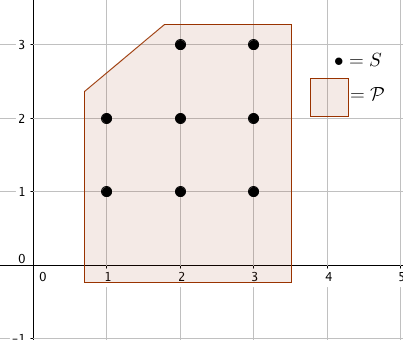
\includegraphics[width=0.25\textwidth]{poliedro}
\caption{La envoltura convexa tiene una cantidad infinita de caras que la definen, y por lo tanto no sería un poliedro.}
\end{figure}
\end{defi}

\begin{defi}[$\mathcal{P}$ es mejor formulación que $\mathcal{Q}$]
Dadas dos fomulaciones $\mathcal{P}$ y $\mathcal{Q}$ de $S$, decimos que $\mathcal{P}$ es mejor que $\mathcal{Q}$ si:
$$
\mathcal{P} \subseteq \mathcal{Q}
$$
\end{defi}
\underline{\textbf{observación}}: Notemos que para toda formulación $\mathcal{P}$ de $S$, siempre se tiene que:
$$
S \subseteq \mathcal{P}
$$
Como además $\mathcal{P}$ es poliedro, podemos concluir que:
$$
\text{conv}(S) \subseteq \mathcal{P}
$$
Así, si ocurriese que $\text{conv}(S)$ fuese un poliedro, entonces sería la mejor formulación.\\

\underline{\textbf{observación}}: $\text{conv}(S)$ no es necesariamente un poliedro. Para ello consideremos el siguiente $S$:
$$
S = \{(x,y) \in \Z^2: y \leq \sqrt{2}x,\ x\geq 1,\ y\geq 1\}
$$

\begin{figure}[h]
\centering
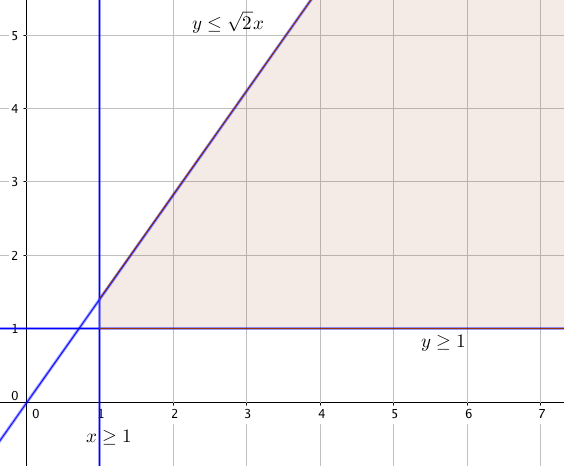
\includegraphics[width=0.25\textwidth]{conv_S}
\caption{La envoltura convexa tiene una cantidad infinita de caras que la definen, y por lo tanto no sería un poliedro.}
\end{figure}
\underline{\textbf{observación}}: 
$$
\begin{array}{cccccc}
\text{PL:} & \text{factible} & + & \text{fn. objetivo acotada} &\imp & \text{se alcanza óptimo}\\
\text{PLM:} & \text{factible} & + & \text{fn. objetivo acotada} & y & \text{ no se alcanza óptimo necesariamente}
\end{array}
$$
Uno de los objetivos del curso es probar que esto no ocurre si los datos son racionales.
\end{document}

%%%%%%%%%%%%%%%%%%%%%%%%%%%%%%%%%%%%%%%%%%%%%%%%%%%%%%%%%%%%%%%%%%%%%%%%%%%%%%%%%%%%%%%%%%%%
%%%%%%%%%%%%%%%%%%%%%%%%%%%%%%%%%%%%%%%%%%%%%%%%%%%%%%%%%%%%%%%%%%%%%%%%%%%%%%%%%%%%%%%%%%%%

